\documentclass[11pt,a4paper]{article}

\usepackage[utf8]{inputenc}
\usepackage[margin=0.5in]{geometry}
\usepackage{xcolor}
\usepackage{tikz}
\usetikzlibrary{shapes.multipart, positioning, arrows.meta, calc}

\pagestyle{empty} % Standalone single page

% Clean UML Color Palette
\definecolor{classHeader}{RGB}{232, 240, 254}
\definecolor{classBorder}{RGB}{26, 115, 232}
\definecolor{traitHeader}{RGB}{230, 244, 234}
\definecolor{traitBorder}{RGB}{19, 115, 51}
\definecolor{excHeader}{RGB}{254, 239, 222}
\definecolor{excBorder}{RGB}{217, 119, 6}

% TikZ UML Styles with explicit formatting
\tikzset{
    umlclass/.style={
        rectangle split,
        rectangle split parts=3,
        rectangle split part fill={classHeader, white, white},
        draw=classBorder,
        line width=0.8pt,
        rounded corners=2pt,
        font=\small\ttfamily,
        inner sep=6pt,
        align=left
    },
    umltrait/.style={
        rectangle split,
        rectangle split parts=2,
        rectangle split part fill={traitHeader, white},
        draw=traitBorder,
        line width=0.8pt,
        rounded corners=2pt,
        font=\small\ttfamily,
        inner sep=6pt,
        align=left
    },
    umlexception/.style={
        rectangle split,
        rectangle split parts=2,
        rectangle split part fill={excHeader, white},
        draw=excBorder,
        line width=0.8pt,
        rounded corners=2pt,
        font=\small\ttfamily,
        inner sep=5pt,
        align=left
    },
    inherits/.style={
        -{Triangle[open, length=8pt, width=6pt]},
        thick,
        draw=black!80
    },
    composition/.style={
        -{Diamond[fill=black, length=8pt, width=6pt]},
        thick,
        draw=black!80
    },
    dependency/.style={
        ->,
        dashed,
        thick,
        draw=black!80
    }
}

\begin{document}

\begin{center}
    {\Large \textbf{UML Class Diagram }}\\[0.2em]

\end{center}

\vspace{0.4em}

\begin{figure}[htbp]
\centering
% Auto-scales cleanly to page margins without any clipping
\resizebox{\textwidth}{!}{
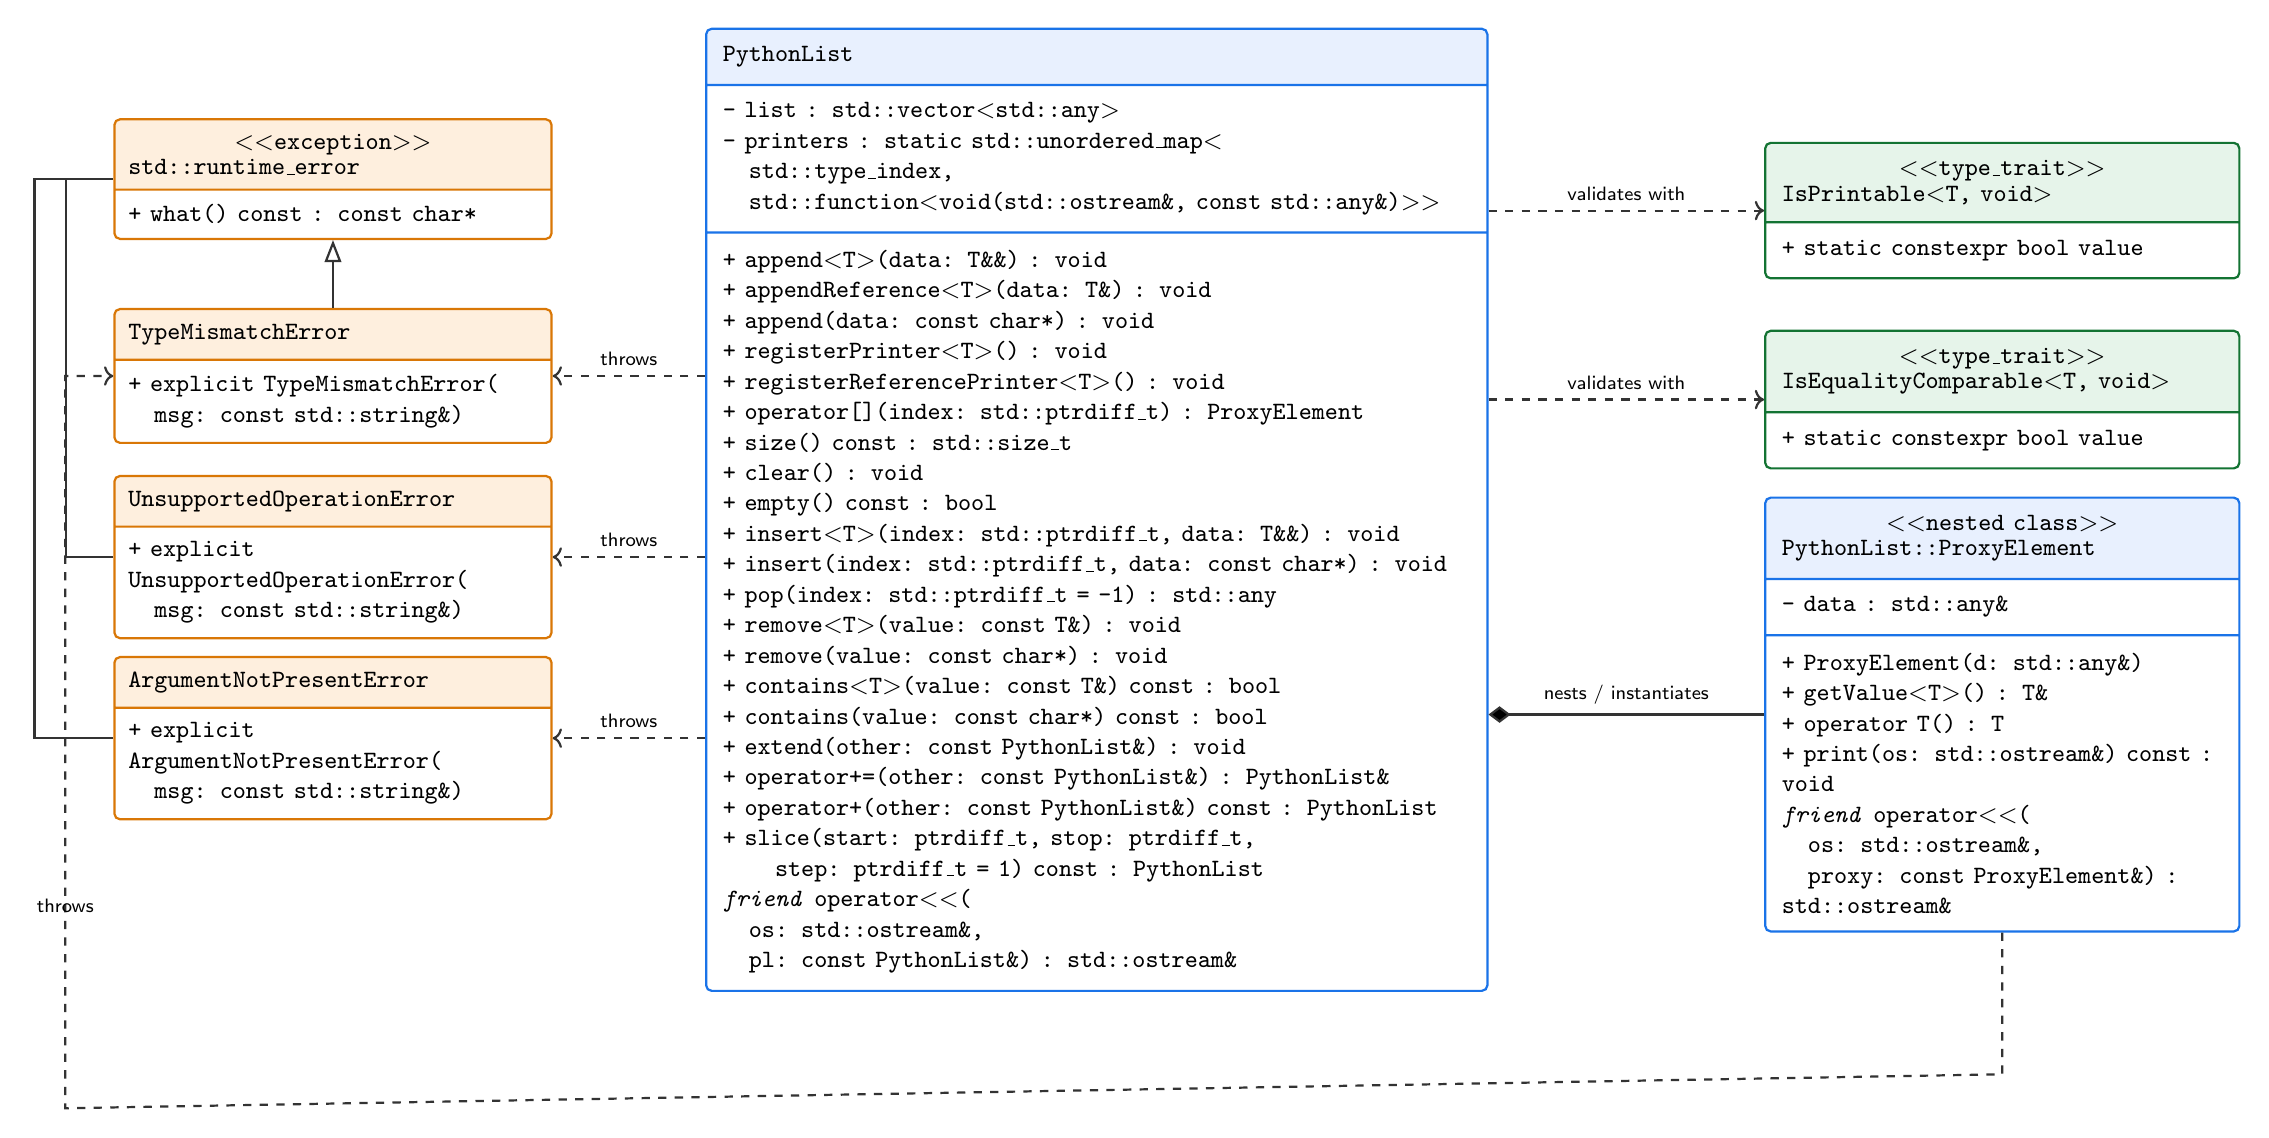
\begin{tikzpicture}[auto]

    % =========================================================================
    % COLUMN 1 (LEFT): EXCEPTION HIERARCHY (Centered at X = -9.2)
    % =========================================================================

    % Base Exception std::runtime_error
    \node (runtime_error) [umlexception, text width=5.2cm] at (-9.2, 4.8) {
        \centering\textbf{\textless\textless exception\textgreater\textgreater}\\[-0.2em]
        \centering\textbf{std::runtime\_error}
        \nodepart{second}
        + what() const : const char*
    };

    % Custom Exception 1: TypeMismatchError
    \node (type_mismatch) [umlexception, text width=5.2cm] at (-9.2, 2.3) {
        \centering\textbf{TypeMismatchError}
        \nodepart{second}
        + explicit TypeMismatchError(\\
        \quad msg: const std::string\&)
    };

    % Custom Exception 2: UnsupportedOperationError
    \node (unsupported_op) [umlexception, text width=5.2cm] at (-9.2, 0.0) {
        \centering\textbf{UnsupportedOperationError}
        \nodepart{second}
        + explicit UnsupportedOperationError(\\
        \quad msg: const std::string\&)
    };

    % Custom Exception 3: ArgumentNotPresentError
    \node (arg_not_present) [umlexception, text width=5.2cm] at (-9.2, -2.3) {
        \centering\textbf{ArgumentNotPresentError}
        \nodepart{second}
        + explicit ArgumentNotPresentError(\\
        \quad msg: const std::string\&)
    };

    % Clean Inheritance Arrows (Direct vertical & outer trunk - NO CROSSING)
    \draw [inherits] (type_mismatch.north) -- (runtime_error.south);
    \draw [thick, draw=black!80] (unsupported_op.west) -- ++(-0.6, 0) |- (runtime_error.west);
    \draw [thick, draw=black!80] (arg_not_present.west) -- ++(-1.0, 0) |- (runtime_error.west);

    % =========================================================================
    % COLUMN 2 (CENTER): MAIN CONTAINER PythonList (Centered at X = 0.5)
    % =========================================================================

    \node (python_list) [umlclass, text width=9.5cm] at (0.5, 0.6) {
        \centering\textbf{PythonList}
        \nodepart{second}
        - list : std::vector\textless std::any\textgreater \\
        - printers : static std::unordered\_map\textless\\
        \quad std::type\_index,\\
        \quad std::function\textless void(std::ostream\&, const std::any\&)\textgreater\textgreater
        \nodepart{third}
        + append\textless T\textgreater(data: T\&\&) : void\\
        + appendReference\textless T\textgreater(data: T\&) : void\\
        + append(data: const char*) : void\\
        + registerPrinter\textless T\textgreater() : void\\
        + registerReferencePrinter\textless T\textgreater() : void\\
        + operator[](index: std::ptrdiff\_t) : ProxyElement\\
        + size() const : std::size\_t\\
        + clear() : void\\
        + empty() const : bool\\
        + insert\textless T\textgreater(index: std::ptrdiff\_t, data: T\&\&) : void\\
        + insert(index: std::ptrdiff\_t, data: const char*) : void\\
        + pop(index: std::ptrdiff\_t = -1) : std::any\\
        + remove\textless T\textgreater(value: const T\&) : void\\
        + remove(value: const char*) : void\\
        + contains\textless T\textgreater(value: const T\&) const : bool\\
        + contains(value: const char*) const : bool\\
        + extend(other: const PythonList\&) : void\\
        + operator+=(other: const PythonList\&) : PythonList\&\\
        + operator+(other: const PythonList\&) const : PythonList\\
        + slice(start: ptrdiff\_t, stop: ptrdiff\_t,\\
        \quad\quad step: ptrdiff\_t = 1) const : PythonList\\
        \textit{friend} operator\textless\textless(\\
        \quad os: std::ostream\&,\\
        \quad pl: const PythonList\&) : std::ostream\&
    };

    % =========================================================================
    % COLUMN 3 (RIGHT): TRAITS & PROXY ELEMENT (Centered at X = 12.0)
    % Generous 4.0cm horizontal channel to PythonList prevents any text collision
    % =========================================================================

    % Compile-time Trait 1: IsPrintable
    \node (is_printable) [umltrait, text width=5.6cm] at (12.0, 4.4) {
        \centering\textbf{\textless\textless type\_trait\textgreater\textgreater}\\[-0.2em]
        \centering\textbf{IsPrintable\textless T, void\textgreater}
        \nodepart{second}
        + static constexpr bool value
    };

    % Compile-time Trait 2: IsEqualityComparable
    \node (is_equality) [umltrait, text width=5.6cm] at (12.0, 2.0) {
        \centering\textbf{\textless\textless type\_trait\textgreater\textgreater}\\[-0.2em]
        \centering\textbf{IsEqualityComparable\textless T, void\textgreater}
        \nodepart{second}
        + static constexpr bool value
    };

    % Nested ProxyElement Class
    \node (proxy_element) [umlclass, text width=5.6cm] at (12.0, -2.0) {
        \centering\textbf{\textless\textless nested class\textgreater\textgreater}\\[-0.2em]
        \centering\textbf{PythonList::ProxyElement}
        \nodepart{second}
        - data : std::any\&
        \nodepart{third}
        + ProxyElement(d: std::any\&)\\
        + getValue\textless T\textgreater() : T\&\\
        + operator T() : T\\
        + print(os: std::ostream\&) const : void\\
        \textit{friend} operator\textless\textless(\\
        \quad os: std::ostream\&,\\
        \quad proxy: const ProxyElement\&) : std::ostream\&
    };

    % =========================================================================
    % CLEAN RELATIONSHIPS & LABELS (SPACIOUS, NO OVERLAPPING TEXT)
    % =========================================================================

    % 1. Exception Throws (Column 2 -> Column 1, with midway labels)
    \draw [dependency] (python_list.west |- type_mismatch.east) -- 
          node[above, midway, font=\scriptsize\sffamily] {throws} (type_mismatch.east);

    \draw [dependency] (python_list.west |- unsupported_op.east) -- 
          node[above, midway, font=\scriptsize\sffamily] {throws} (unsupported_op.east);

    \draw [dependency] (python_list.west |- arg_not_present.east) -- 
          node[above, midway, font=\scriptsize\sffamily] {throws} (arg_not_present.east);

    % 2. Type Trait Validations (Wide 4cm channel ensures labels never touch boxes)
    \draw [dependency] (python_list.east |- is_printable.west) -- 
          node[above, midway, font=\scriptsize\sffamily] {validates with} (is_printable.west);

    \draw [dependency] (python_list.east |- is_equality.west) -- 
          node[above, midway, font=\scriptsize\sffamily] {validates with} (is_equality.west);

    % 3. Composition with ProxyElement (Wide channel ensures label is fully isolated)
    \draw [composition] (proxy_element.west) -- 
          node[above, midway, font=\scriptsize\sffamily] {nests / instantiates} (python_list.east |- proxy_element.west);

    % 4. ProxyElement Throws TypeMismatchError (Outer perimeter path well below PythonList)
    \draw [dependency] (proxy_element.south) -- ++(0, -1.8) -- (-12.6, -7.0) |- 
          node[pos=0.15, below, font=\scriptsize\sffamily] {throws} (type_mismatch.west);

\end{tikzpicture}
}
\end{figure}

\end{document}
